\documentclass[varwidth=true, border=2pt]{standalone}

\usepackage{pgfplots}
\usepackage{tikz}

\usetikzlibrary{calc,patterns,angles,quotes}

\begin{document}
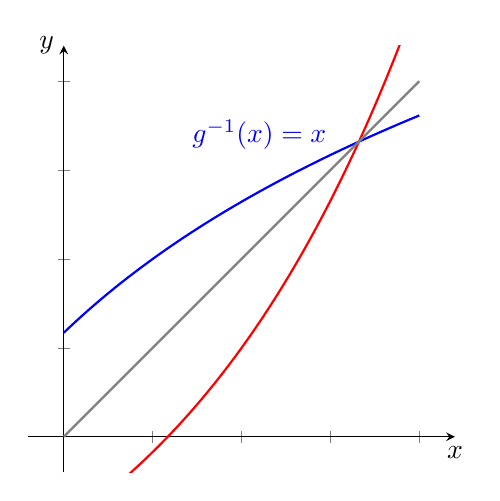
\begin{tikzpicture}
    \begin{axis}[
        legend pos=south east,
        axis x line=middle,
        axis y line=middle,
	every axis x label/.style={at={(current axis.right of origin)},anchor=north},
	every axis y label/.style={at={(current axis.above origin)},anchor=east},
	xticklabels=\empty,
	yticklabels=\empty
        grid = none ,
        width=7cm,
        height=7cm,
        grid style={dashed, gray!1},
        xmin=0,     % start the diagram at this x-coordinate
        xmax= 2,    % end   the diagram at this x-coordinate
        ymin=0,     % start the diagram at this y-coordinate
        ymax= 2,   % end   the diagram at this y-coordinate
        xlabel=$x$,
        ylabel=$y$,
        enlargelimits=true,
        tension=0.08]

        \addplot[domain=-0:2,blue, thick,samples=250] {log2(x+1.5)};
        \addplot[domain=-0:2,red, thick,samples=250] {pow(2,x)-1.5};
         \addplot[domain=-0:2, gray, thick,samples=250] {x};

	\node[blue] (x0) at (axis cs: 1.1,1.7){$g^{-1}(x)=x$};

    \end{axis}
\end{tikzpicture}
\end{document}